\documentclass[]{article}
\usepackage{ctex,hyperref}% 输出汉字
\usepackage{amsmath,amssymb,amsfonts}
\usepackage{amsthm,amsmath,amssymb}
\usepackage{mathrsfs}
%opening
\usepackage{setspace}
\usepackage{lipsum}
\usepackage{graphicx}% 图片插入宏包
\usepackage{subfigure}% 并排子图
\usepackage{float}% 浮动环境,用于调整图片位置
\usepackage[export]{adjustbox}% 防止过宽的图片
\usepackage{amsmath}
\usepackage{extarrows}
\graphicspath{{Figures/}}%文章所用图片在当前目录下的 Figures目录
\usepackage{hyperref} %生成引用链接
\usepackage{cleveref} %实现图片和表格、公式的引用
%%链接设置
\hypersetup{colorlinks = false}
\title{角动量}
\author{步允霆}

\begin{document}
	
	\maketitle
	\tableofcontents
\section{角动量与对易关系}
\subsection{轨道角动量}
经典角动量为
\begin{equation}
	\mathscr{L}_x=yp_z-zp_y
\end{equation}
根据量子化规则
\begin{equation}
	L_x=YP_z-ZP_y
\end{equation}
如此构造的算符是厄米算符。\par 
按相同的办法可以得到与经典角动量分量$\mathscr{L}_y,\mathscr{L}_z$对应的算符$L_y,L_z$;于是,我们可以写成
\begin{equation}
	\mathbf{L}=\mathbf{R}\times\mathbf{P}
\end{equation}

接下来计算对易子$[L_x,L_y]$
\begin{align}
	[L_x,L_y]&=[YP_z-ZP_y,ZP_x-XP_z]\nonumber\\
	&=[YP_z,ZP_x]+[ZP_y,XP_z]
\end{align}
于是我们有
\begin{align}
	[L_z,L_y]&=Y[P_z,Z]P_x+X[Z,P_z]P_y\nonumber\\
	&=-\mathrm{i}\hbar YP_x+\mathrm{i}\hbar XP_y\nonumber\\
	&=\mathrm{i}\hbar L_z
\end{align}
类似的,可以给出其他对易子
\begin{align}
	[L_x,L_y]&=\mathrm{i}\hbar L_z\nonumber\\
	[L_y,L_z]&=\mathrm{i}\hbar L_x\nonumber\\
	[L_z,L_x]&=\mathrm{i}\hbar L_y
	\label{b6b6}
\end{align}
这样,我们建立了一个无自旋粒子的角动量诸分量之间的对易关系式。\par 
上述结果可以推广至$N$个无自旋粒子的体系。在量子力学中,这个体系的总角动量就是
\begin{equation}
	\mathbf{L}=\sum\limits_{i=1}^{N}\mathbf{L}_i
\end{equation}
其中
\begin{equation}
	\mathbf{L}_i=\mathbf{R}_i\times\mathbf{P}_i
\end{equation}
每一个粒子的角动量$\mathbf{L}_i$都满足对易关系\eqref{b6b6},而且只要$j$不同于$i$,他就可以和$\mathbf{L}_j$对易。
\subsection{角动量定义的推广}
如果任意三个观察算符$J_x,J_y,J_z$满足如下关系式
\begin{align}
	[J_x,J_y]&=\mathrm{i}\hbar J_z\nonumber\\
	[J_y,J_z]&=\mathrm{i}\hbar J_x\nonumber\\
	[J_z,J_x]&=\mathrm{i}\hbar J_y	
	\label{b9b9}
\end{align}
我们就称$J_x,J_y,J_z$的集合为角动量$\boldsymbol{J}$。\par 
我们现在引入角动量$\boldsymbol{J}$的平方的算符
\begin{equation}
	\boldsymbol{J}^2=J_x^2+J_y^2+J_z^2
	\label{b10b10}
\end{equation}
因为$J_x,J_y,J_z$都是厄米算符,故$\boldsymbol{J}^2$也是厄米算符。$\boldsymbol{J}^2$与$\boldsymbol{J}$的三个分量对易
\begin{equation}
	[\boldsymbol{J}^2,\boldsymbol{J}]=0
	\label{b11b11}
\end{equation}
以$J_x$为例证明如下
\begin{align}
	[\boldsymbol{J}^2,J_x]&=[J_x^2+J_y^2+J_z^2,J_x]\nonumber\\
	&=[J_y^2,J_x]+[J_z^2,J_x]
	\label{b12b12}
\end{align}
根据\eqref{b9b9},很容易算出其他两个对易子
\begin{subequations}
	\begin{align}
		[J_y^2,J_x]&=J_y[J_y,J_x]+[J_y,J_x]J_y\nonumber\\
		&=-\mathrm{i}\hbar J_yJ_z-\mathrm{i}\hbar J_zJ_y
	\end{align}
	\begin{align}
		[J_z^2,J_x]&=J_z[J_z,J_x]+[J_z,J_x]J_z\nonumber\\
		&=-\mathrm{i}\hbar J_zJ_y-\mathrm{i}\hbar J_yJ_z
	\end{align}
\end{subequations}
由此可见,\eqref{b12b12}中的两个对易子之和等于零。\par 
量子力学的角动量理论完全建立在对易关系\eqref{b9b9}的基础上,意味着:角动量的三个分量是不可能同时测量的,但是,$\boldsymbol{J}^2$与$\boldsymbol{J}$的任意一个分量却都是相容的。
\section{角动量的普遍理论}
\subsection{定义与符号}
\subsubsection{算符$J_+$和$J_-$}
不使用角动量$\boldsymbol{J}$的分量$J_x$和$J_y$而引入他们的线性组合,将是方便的
\begin{align}
	J_+&=J_x+\mathrm{i}J_y\nonumber\\
	J_-&=J_x-\mathrm{i}J_y
	\label{c1c1}
\end{align}
与谐振子$a$和$a^\dagger$相似,$J_+,J_-$不是厄米算符,但他们互为伴随算符。\par 
根据\eqref{b9b9}\eqref{b11b11},很容易证明这些算符满足下列对易关系:
\begin{equation}
	[J_z,J_+]=\hbar J_+
\end{equation}
\begin{equation}
	[J_z,J_-]=-\hbar J_-
\end{equation}
\begin{equation}
	[J_+,J_-]=2\hbar J_z
\end{equation}
\begin{equation}
	[\boldsymbol{J}^2,J_+]=[\boldsymbol{J}^2,J_-]=[\boldsymbol{J}^2,J_z]=0
\end{equation}
我们来计算$J_+J_-$和$J_-J_+$
\begin{align}
	J_+J_-&=(J_x+\mathrm{i}J_y)(J_x-\mathrm{i}J_y)\nonumber\\
	&=J_x^2+J_y^2-\mathrm{i}[J_x,J_y]\nonumber\\
	&=J_x^2+J_y^2+\hbar J_z
\end{align}
\begin{align}
	J_-J_+&=(J_x-\mathrm{i}J_y)(J_x+\mathrm{i}J_y)\nonumber\\
	&=J_x^2+J_y^2+\mathrm{i}[J_x,J_y]\nonumber\\
	&=J_x^2+J_y^2-\hbar J_z
\end{align}
应用定义$\boldsymbol{J}^2$的\eqref{b10b10},还可以把这些式子写成下列形式
\begin{subequations}
	\begin{equation}
		J_+J_-=\boldsymbol{J}^2-J_z^2+\hbar J_z
	\end{equation}
	\begin{equation}
	J_-J_+=\boldsymbol{J}^2-J_z^2-\hbar J_z
	\end{equation}
\label{c7c7}
\end{subequations}
将此两式的对应项相加,便可得
\begin{equation}
	\boldsymbol{J}^2=\dfrac{1}{2}(J_+J_-+J_-J_+)+J_z^2
\end{equation}
\subsubsection{$\boldsymbol{J}^2$与$J_z$的本征值符号与方程}
根据\eqref{b10b10},$\boldsymbol{J}^2$是三个厄米算符的平方之和,因而不论$|\varphi\rangle$是任何右矢,矩阵元$\langle\varphi|\boldsymbol{J}^2|\varphi\rangle$总是整数或零:
\begin{align}
	\langle\varphi|\boldsymbol{J}^2|\varphi\rangle&=\langle\varphi|J_x^2|\varphi\rangle+\langle\varphi|J_y^2|\varphi\rangle+\langle\varphi|J_z^2|\varphi\rangle\nonumber\\
	&\parallel J_x|\varphi\rangle\parallel^2+\parallel J_y|\varphi\rangle\parallel^2+\parallel J_z|\varphi\rangle\parallel^2\geqslant0
\end{align}
我们可以由此推知:$\boldsymbol{J}^2$的全体本征值都是整数或零,这是因为,如果$|\varphi\rangle$是$\boldsymbol{J}^2$的本征矢,那么,$\langle\varphi|\boldsymbol{J}^2|\varphi\rangle$就是对应的本征值与$|\varphi\rangle$的模平方的乘积。\par 
我们把:$\boldsymbol{J}^2$的本征值写成$j(j+1)\hbar^2$的形式,并且按照惯例取
\begin{equation}
	j\geqslant0
	\label{c10c10}
\end{equation}
引入这个符号的目的在于简化以后的推证。由于$\boldsymbol{J}$具有$\hbar$的量纲,故$\boldsymbol{J}^2$的任何本征值都具有$\lambda\hbar$的形式,其中的$\lambda$是一个无量纲的实数。我们刚才看到,$\lambda$一个是正数或零;于是很容易证明关于$j$的二次方程
\begin{equation}
	j(j+1)=\lambda
\end{equation}
必有而且只有一个正的或等于零的根。如果加上条件\eqref{c10c10}的限制,那么,$\lambda$的值就唯一确定了$j$的值;因此,$\boldsymbol{J}^2$的任一本征值都可以写作$j(j+1)\hbar^2$的形式,其中$j$是正数或零。\par 
至于$J_z$的本征值,其量纲和$\hbar$的相同,习惯上,我们将这些本征值记作$m\hbar$,其中$m$是无量纲的数。\par 
我们将用确定$\boldsymbol{J}^2$与$J_z$的本征值的指标$j$和$m$来标记此两算符的共同本征矢。但是,一般来说,$\boldsymbol{J}^2$和$J_z$并不构成一个CSCO,因而必须引入第三个指标,用来区别对应于$\boldsymbol{J}^2$的同一本征值$j(j+1)\hbar^2$和$J_z$的同一本征值$m\hbar$的那些不同的本征矢,我们将这个指标记作$k$。\par 
这样一来,我们试图求解的本征值方程组便成为
\begin{align}
	\boldsymbol{J}^2|k,j,m\rangle&=j(j+1)\hbar^2|k,j,m\rangle\nonumber\\
	J_z|k,j,m\rangle&=m\hbar|k,j,m\rangle
	\label{c12c12}
\end{align}
\subsection{$\boldsymbol{J}^2$与$J_z$的本征值}
\subsubsection{引理1:$\boldsymbol{J}^2$与$J_z$本征值的性质}
如果$j(j+1)\hbar^2$与$m\hbar$是$\boldsymbol{J}^2$与$J_z$的对应于同一本征矢$|k,j,m\rangle$的本征值,则$j$与$m$满足下列不等式
\begin{equation}
	-j\leqslant m\leqslant j
	\label{c13c13}
\end{equation}

我们来考虑矢量$J_+|k,j,m\rangle$与$J_-|k,j,m\rangle$,他们的模平方为正值或零,即
\begin{subequations}
	\begin{equation}
		\parallel J_+|k,j,m\rangle\parallel^2=\langle k,j,m|J_-J_+|k,j,m\rangle\geqslant0
	\end{equation}
	\begin{equation}
		\parallel J_-|k,j,m\rangle\parallel^2=\langle k,j,m|J_+J_-|k,j,m\rangle\geqslant0
	\end{equation}
\label{c14c14}
\end{subequations}
为了计算这些不等式的左端,我们可以利用\eqref{c7c7},并且假定$|k,j,m\rangle$已经归一化,这样便有
\begin{subequations}
	\begin{align}
		\langle k,j,m|J_-J_+|k,j,m\rangle&=\langle k,j,m|(\boldsymbol{J}^2-J_z^2-\hbar J_z)|k,j,m\rangle\nonumber\\
		&=j(j+1)\hbar^2-m^2\hbar^2-m\hbar^2
	\end{align}
	\begin{align}
		\langle k,j,m|J_+J_-|k,j,m\rangle&=\langle k,j,m|(\boldsymbol{J}^2-J_z^2+\hbar J_z)|k,j,m\rangle\nonumber\\
		&=j(j+1)\hbar^2-m^2\hbar^2+m\hbar^2
	\end{align}
\end{subequations}
将这些结果代入不等式\eqref{c14c14},得到
\begin{subequations}
	\begin{equation}
		j(j+1)-m(m+1)=(j-m)(j+m+1)\geqslant0
	\end{equation}
	\begin{equation}
		j(j+1)-m(m-1)=(j-m+1)(j+m)\geqslant0
	\end{equation}
\end{subequations}
亦即
\begin{subequations}
	\begin{equation}
		-(j+1)\leqslant m\leqslant j
	\end{equation}
	\begin{equation}
		-j\leqslant m\leqslant j+1
	\end{equation}
\end{subequations}
仅当$m$满足不等式\eqref{c13c13}时,这两个条件才能同时满足。
\subsubsection{引理2:矢量$J_-|k,j,m\rangle$的性质}
设$|k,j,m\rangle$是$\boldsymbol{J}^2$与$J_z$的一个本征矢,属于本征值$j(j+1)\hbar^2$与$m\hbar$。\par 
(1)如果$m=-j$。则$J_-|k,j,-j\rangle=0$。\par 
(2)如果$m>-j$,则$J_-|k,j,m\rangle$是$\boldsymbol{J}^2$与$J_z$的一个非零本征矢,属于本征值$j(j+1)\hbar^2$与$(m-1)\hbar$。\par 
两个性质的证明分别使用对易子$[\boldsymbol{J}^2,J_-]$与$[J_z,J_-]$即可。
\subsubsection{引理3:矢量$J_+|k,j,m\rangle$的性质}
设$|k,j,m\rangle$是$\boldsymbol{J}^2$与$J_z$的一个本征矢,属于本征值$j(j+1)\hbar^2$与$m\hbar$。\par 
(1)如果$m=j$。则$J_+|k,j,j\rangle=0$。\par 
(2)如果$m<j$,则$J_+|k,j,m\rangle$是$\boldsymbol{J}^2$与$J_z$的一个非零本征矢,属于本征值$j(j+1)\hbar^2$与$(m-1)\hbar$。\par 
证明方法与上节相似。
\subsubsection{确定$\boldsymbol{J}^2$及$J_z$的谱}
设$|k,j,m\rangle$是$\boldsymbol{J}^2$和$J_z$的一个非零本征矢,属于本征值$j(j+1)\hbar^2$与$m\hbar$。那么,根据引理1,应该有$-j\leqslant m\leqslant j$。因而,一定存在一个非负的整数$p$使得
\begin{equation}
	-j\leqslant m-p<-j+1
	\label{c29c29}
\end{equation}
考虑下面的矢量序列
\begin{equation}
	|k,j,m\rangle,J_-|k,j,m\rangle,\cdots,(J_-)^p|k,j,m\rangle
	\label{c30c30}
\end{equation}
根据引理2,此序列中的每一个矢量$(J_-)^p|k,j,m\rangle(n=0,1,\cdots,p)$都是$\boldsymbol{J}^2$与$J_z$的非零本征矢,属于本征值$j(j+1)\hbar^2$与$m\hbar$。\par 
我们逐步的证明:根据假设,$|k,j,m\rangle$是一个非零矢量,属于本征值$j(j+1)\hbar^2$与$m\hbar$;将算符$J_-$作用于矢量$(J_-)^{n-1}|k,j,m\rangle$,便得到矢量$(J_-)^n|k,j,m\rangle$,前一个矢量是$\boldsymbol{J}^2$与$J_z$的本征矢,属于本征值$j(j+1)\hbar^2$与$(m-n+1)\hbar$;后面这个本征值是严格大于$-j\hbar$的,这是因为,根据\eqref{c29c29}有
\begin{equation}
	m-n+1\geqslant m-p+1\geqslant-j+1
\end{equation}
根据引理2的第(2)点,可知$(J_-)^n|k,j,m\rangle$是$\boldsymbol{J}^2$与$J_z$的非零本征矢,属于本征值$j(j+1)\hbar^2$与$(m-n)\hbar$。\par 
现在将算符$J_-$作用于$(J_-)^p|k,j,m\rangle$。首先假设$J_z$的与矢量$(J_-)^p|k,j,m\rangle$相联系的本征值$(m-p)\hbar$严格大于$-j\hbar$,也就是说
\begin{equation}
	m-p>-j
\end{equation}
根据引理2的第(2)点,$J_-(J_-)^p|k,j,m\rangle$就应该是一个非零矢量而且应该对应于本征值$j(j+1)\hbar^2$与$(m-p-1)\hbar$,这就和引理1互相矛盾了;这是因为,根据\eqref{c29c29},有
\begin{equation}
	m-p-1<-j
\end{equation}

因而$m-p$必须等于$-j$。在这个条件下,$(J_-)^p|k,j,m\rangle$实际上对应于$J_z$的本征值$-j\hbar$,而且,根据引理2的第(2)点,$J_-(J_-)^p|k,j,m\rangle$是个零矢量;因而,通过算符$J_-$迭次作用于$|k,j,m\rangle$而形成的矢量序列\eqref{c30c30}是有限的,而且与引理1的矛盾也消除了。\par 
于是我们证明了:存在着这样一个整数$p$,他取正值或零,使得
\begin{equation}
	m-p=-j
	\label{c34c34}
\end{equation}

和上面完全相同的推理可以证明:根据引理3,存在这样一个整数$q$,他取正值或零,使得
\begin{equation}
	m+q=j
	\label{c35c35}
\end{equation}
这是因为矢量序列
\begin{equation}
	|k,j,m\rangle,J_+|k,j,m\rangle,\cdots,(J_+)^p|k,j,m\rangle
	\label{c36c36}
\end{equation}
必须是有限的,才不致和引理1矛盾。\par 
将\eqref{c34c34}\eqref{c35c35}结合起来,我们得到
\begin{equation}
		p+q=2j
\end{equation}
因而$j$等于正整数的一半或零。由此可以推知,$j$必须是整数或半整数。此外,如果存在一个非零矢量$|k,j,m\rangle$,则序列\eqref{c30c30}\eqref{c36c36}中的所有矢量也都是非零矢量;而且都是$\boldsymbol{J}^2$的属于本征值$j(j+1)\hbar^2$的本征矢又都是$J_z$的属于本征值
\begin{equation}
	-j\hbar,(-j+1)\hbar,(-j+2)\hbar,\cdots,(j-2)\hbar,(j-1)\hbar,j\hbar 
\end{equation}
的本征矢。\par 
现在把结果归纳如下\par 
假设$\boldsymbol{J}$是满足对易关系式\eqref{b9b9}的任意角动量。如果$j(j+1)\hbar^2$与$m\hbar$表示$\boldsymbol{J}^2$与$J_z$的本征值,那么\par 
(1)$\quad j$只能取正的整数、半整数或零,即$0,1/2,1,3/2,2,\cdots$\par 
(2)对于$j$的一个固定值,$m$的可能值只有$(2j+1)$个:$-j,-j+1,\cdots,j-1,j$。因此,若$j$是半整数,则$m$也是半整数。在$m$的这些值中,只要有一个出现,其他的值也会出现。
\subsection{表象${|k,j,m\rangle}$}
\subsubsection{基右矢}
我们取在所研究的情况下能够出现一对本征值$j(j+1)\hbar^2$与$m\hbar$。与这一对本征值相联系的本征矢的集合在$\mathscr{E}$空间中张成一个矢量子空间,我们将他记作$\mathscr{E}(j,m)$;可以预见他的维数$g(j,m)$大于1,这是因为一般来说$\boldsymbol{J}^2$与$J_z$并不构成一个CSCO。现在,我们在子空间$\mathscr{E}(j,m)$中选择一个任意的正交归一基${|k,j,m\rangle;k=1,2,\cdots,g(j,m)}$。\par 
如果$m$不等于$j$,则在$\mathscr{E}$空间中一定有另一个子空间$\mathscr{E}(j,m+1)$,他由$\boldsymbol{J}^2$与$J_z$的属于本征值$j(j+1)\hbar^2$与$m\hbar$的本征矢所张成。同样,若$m$不等于$-j$,便存在着一个子空间$\mathscr{E}(j,m-1)$。我们从$\mathscr{E}(j,m)$空间中已经选定的基出发,在$m$不等于$j$与$-j$的情况下,在$\mathscr{E}(j,m+1)$空间和$\mathscr{E}(j,m-1)$空间中构成一个正交归一基。\par 
首先,我们证明,若$k_1$不等于$k_2$,则$J_+|k_1,j,m\rangle$与$J_+|k_2,j,m\rangle$正交;$J_-|k_1,j,m\rangle$与$J_-|k_2,j,m\rangle$也是正交的。我们利用\eqref{c7c7}来计算$J_{\pm}|k_2,j,m\rangle$和$J_{\pm}|k_1,j,m\rangle$的标量积
\begin{align}
	\langle k_2,j,m|J_{\mp}J_{\pm}|k_1,j,m\rangle&=\langle k_2,j,m|(\boldsymbol{J}^2-J_z^2\mp\hbar J_z)|k_1,j,m\rangle\nonumber\\
	&=[j(j+1)-m(m\pm1)]\hbar^2\langle k_2,j,m|k_1,j,m\rangle
\end{align}
由于$\mathscr{E}(j,m)$空间中的基是正交归一的,如果$k_1\neq k_2$,则这些标量积都是零。如果$k_1=k_2$,便得到矢量$J_{\pm}|k,j,m\rangle$的模平方$[j(j+1)-m(m\pm1)]\hbar^2$。\par 
现在,我们来考虑由下式
\begin{equation}
	|k,j,m+1\rangle=\dfrac{1}{\hbar\sqrt{j(j+1)-m(m+1)}}J_+|k,j,m\rangle
	\label{c40c40}
\end{equation}
定义是$g(j,m)$个矢量的集合。根据上面的论证,这些矢量是正交归一的。此外,他们构成$\mathscr{E}(j,m+1)$空间中的一个基。这一点可证明如下:我们假设在$\mathscr{E}(j,m+1)$空间中存在一个矢量$|\alpha,j,m+1\rangle$,他正交于自\eqref{c40c40}的全体矢量$|k,j,m+1\rangle$。因为$m+1$不会等于$-j$,故矢量$J_-|\alpha,j,m+1\rangle$不会是零矢量,他应该属于$\mathscr{E}(j,m)$,并应正交于所有的矢量$J_-|k,j,m+1\rangle$;但根据\eqref{c40c40},$J_-|k,j,m+1\rangle$正比于$J_-J_+|k,j,m\rangle$,即正比于$|k,j,m\rangle$;于是$J_-|\alpha,j,m+1\rangle$应是$\mathscr{E}(j,m)$空间中的一个非零矢量,他正交于基${|k,j,m\rangle}$中的所有矢量,但这是不可能的。因而矢量集合\eqref{c40c40}构成$\mathscr{E}(j,m+1)$空间中的一个基。\par 
采用和上面完全相同的方法,我们可以证明:由下式定义的诸矢量$|k,j,m-1\rangle$
\begin{equation}
	|k,j,m-1\rangle=\dfrac{1}{\hbar\sqrt{j(j+1)-m(m-1)}}J_-|k,j,m\rangle
	\label{c41c41}
\end{equation}
构成$\mathscr{E}(j,m-1)$空间中的一个正交归一基。\par 
特别的,我们看到,子空间$\mathscr{E}(j,m+1)$和子空间$\mathscr{E}(j,m-1)$的维数等于$\mathscr{E}(j,m)$空间的维数。换句话说,他们的维数与$m$无关
\begin{equation}
	g(j,m+1)=g(j,m-1)=g(j,m)=g(j)
\end{equation}

我们现在按下列步骤进行。对于在待研究的问题中实际出现的$j$的每一个数值。我们取与$j$的数值相联系的诸子空间中的一个。譬如$\mathscr{E}(j,j)$,他对应于$m=j$。我们在这个子空间中任意取一个正交归一基${|k,j,j\rangle;k=1,2,\cdots,g(j)}$,然后,根据\eqref{c41c41},我们可以顺序地为其他$2j$个子空间$\mathscr{E}(j,m)$中的每一个构成一个基。图1中的箭头概略地表示我们所用的方法。对于问题中实际出现的$j$的每一个数值,我们都按照同样的方法去做,最后构成的基叫做态空间$\mathscr{E}$中的标准基。对于这样一个基,正交归一关系式及封闭性关系式可以写作
\begin{subequations}
	\begin{equation}
		\langle k,j,m|k^\prime,j^\prime,m^\prime\rangle=\delta_{kk^\prime}\delta_{jj^\prime}\delta_{mm^\prime}
	\end{equation}
	\begin{equation}
		\sum\limits_{j}\sum\limits_{m=-j}^{+j}\sum\limits_{k=1}^{g(j)}|k,j,m\rangle\langle k,j,m|=1
	\end{equation}
\end{subequations}
\begin{figure}[H]
	\centering
	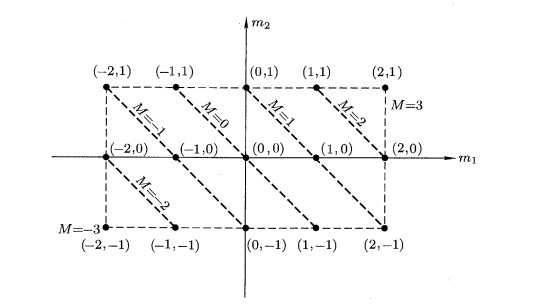
\includegraphics[scale=0.2]{1.png}
	\caption{对于固定$j$,构建标准基}
	\label{Figure 1}
\end{figure}
\subsubsection{子空间$\mathscr{E}(k,j)$}
在上一节中,我们从子空间$\mathscr{E}(j,m=j)$中已选定的一个基出发,构成子空间$\mathscr{E}(j,m=j-1)$中的一个基,然后构成子空间$\mathrm{E}(j,m=j-2),\cdots,\mathscr{E}(j,m),\cdots$中的基,最后便构成态空间中的一个“标准基”。我们可以把态空间看做全体正交子空间$\mathscr{E}(j,m)$的直和,这里$m$从$-j$变到$+j$,每次改变一个单位,而$j$则取遍待研究问题中实际出现的所有数值。这就是说,$\mathscr{E}$空间中的任一个矢量都可以唯一的分解为一系列矢量之和,其中每一个矢量分别属于一个确定的子空间$\mathscr{E}(j,m)$。\par 
但是,利用这些子空间$\mathscr{E}(j,m)$也有不便的地方。首先,他的维数$g(j)$事先是不知道的,而且是与待研究物理体系相关联的;其次,这些子空间$\mathscr{E}(j,m)$在$\boldsymbol{J}$的作用下并不是不变的,这是因为,按照矢量$|k,j,m\rangle$的构成方法,算符$J_+$和$J_-$在子空间$\mathscr{E}(j,m)$的矢量和$\mathscr{E}(j,m\pm1)$的矢量之间的矩阵元并不等于零。\par 
现在我们引入$\mathscr{E}$空间中的另外一些子空间,即子空间$\mathscr{E}(k,j)$。为此,我们不再组合指标$j$和$m$都是固定数值的那些矢量$|k,j,m\rangle$,而另外组成一个集合,其中诸矢量的指标$k$和$j$都具有指定值,我们称这些矢量所张成的空间为子空间$\mathscr{E}(k,j)$。这种做法相当于将图1中的同一列中的$(2j+1)$个矢量[而不是同一行中的$g(j)$个矢量]组合起来。\par 
于是$\mathscr{E}$空间就成为这些正交子空间$\mathscr{E}(k,j)$的直和,现在这些子空间具有如下简单性质\par 
——无论待研究的是什么物理体系,也无论$k$的值如何,子空间$\mathscr{E}(k,j)$的维数都是$(2j+1)$。\par 
——子空间$\mathscr{E}(k,j)$在$\boldsymbol{J}$的作用下具有整体不变性;也就是说,将$\boldsymbol{J}$的任意一个分量$J_u$作用于子空间$\mathscr{E}(k,j)$中的一个右矢,所得的另一个右矢仍属于$\mathscr{E}(k,j)$。这一点是不难证明的,因为$J_u$总可以通过$J_z,J_+$及$J_-$来表示;但由$J_z$对$|k,j,m\rangle$作用而得的右矢正比于$|k,j,m\rangle$,由$J_+$的作用而得的右矢正比于$|k,j,m+1\rangle$,由$J_-$的作用而得的右矢正比于$|k,j,m-1\rangle$;因此,根据构成“标准基”${|k,j,m\rangle}$的方法便可得出上述性质。
\subsubsection{表示角动量算符的矩阵}
在一个标准基中,表示$\boldsymbol{J}$的某一分量$J_u$的矩阵的求法,由于使用子空间$\mathscr{E}(k,j)$而得到很大的简化,实际上,在分别属于互异子空间$\mathscr{E}(k,j)$的两个基右矢之间的矩阵元都等于零。因此,这种矩阵的形式如下
\begin{figure}[H]
	\centering
	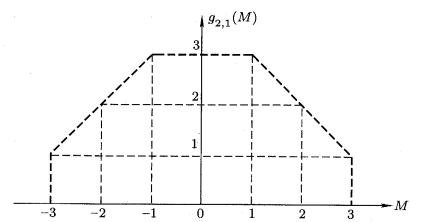
\includegraphics[scale=0.2]{2.png}
	\caption{角动量算符的矩阵}
	\label{Figure 2}
\end{figure}
由此可见,我们只需计算有限阶的子矩阵,在每一个子空间$\mathscr{E}(k,j)$内部,这些矩阵都表示我们所有的算符。\par 
第二个十分重要的简化在于:每一个这样的有限阶子矩阵都不依赖于$k$,也不依赖于待研究体系,而只依赖于$j$;当然,还依赖于我们所要表示的算符。实际上,由$|k,j,m\rangle$的定义,可以推知
\begin{align}
	J_z|k,j,m\rangle&=m\hbar|k,j,m\rangle\nonumber\\
	J_+|k,j,m\rangle&=\hbar\sqrt{j(j+1)-m(m+1)}|k,j,m+1\rangle\nonumber\\
	J_-|k,j,m\rangle&=\hbar\sqrt{j(j+1)-m(m-1)}|k,j,m-1\rangle
	\label{c50c50}
\end{align}
这就是说
\begin{align}
	\langle k,j,m|J_z|k^\prime,j^\prime,m^\prime\rangle&=m\hbar\delta_{kk^\prime}\delta_{jj^\prime}\delta_{mm^\prime}\nonumber\\
	\langle k,j,m|J_\pm|k^\prime,j^\prime,m^\prime\rangle&=\hbar\sqrt{j(j+1)-m^\prime(m^\prime\pm1)}\delta_{kk^\prime}\delta_{jj^\prime}\delta_{mm^\prime\pm1}
	\label{c51c51}
\end{align}
这些等式表明,表示$\boldsymbol{J}$的分量的那些矩阵元只依赖于$j$和$m$,不依赖于$k$。\par 
因此,不论在什么情况下,为了求得在一个标准基中与任意分量$J_u$相联系的矩阵,我们只需对于$j$的所有可能值$(j=0,12,1,3/2,\cdots)$一次算出所有“普适”矩阵$(J_u)^{(j)}$,这些矩阵在子空间$\mathscr{E}(k,j)$内都表示$J_u$。研究一个具体的物理体系与他的角动量$\boldsymbol{J}$时,我们应该确定这个问题中$j$实际上取哪些数值,以及与$j$的每一个数值相联系的子空间$\mathscr{E}(k,j)$的个数$g(j)$[也就是说,他的维数为$(2j+1)g(j)$];我们知道在这种特殊情况下,表示$J_u$的矩阵具有分块对角的形式,即图2,因而,我们可以从刚才定义的普适矩阵出发构成这个矩阵;对于$j$的每一个值,将有$g(j)$个与$(J_u)^{(j)}$全同的子块。\par 
$j$取任意值时,利用\eqref{c51c51}\eqref{c1c1},我们可以写作
\begin{align}
	\langle k,j,&m|J_x|k^\prime,j^\prime,m^\prime\rangle=\dfrac{\hbar}{2}\delta_{kk^\prime}\delta_{jj^\prime}[\sqrt{j(j+1)-m^\prime(m^\prime+1)}\delta_{mm^\prime+1}+\nonumber\\
	&\sqrt{j(j+1)-m^\prime(m^\prime-1)}\delta_{mm^\prime-1}]
\end{align}
\begin{align}
	\langle k,j,&m|J_y|k^\prime,j^\prime,m^\prime\rangle=\dfrac{\hbar}{2\mathrm{i}}\delta_{kk^\prime}\delta_{jj^\prime}[\sqrt{j(j+1)-m^\prime(m^\prime+1)}\delta_{mm^\prime+1}+\nonumber\\
	&\sqrt{j(j+1)-m^\prime(m^\prime-1)}\delta_{mm^\prime-1}]
\end{align}
由此可见,矩阵$(J_z)^{(j)}$是对角的,他的元是$m\hbar$的$(2j+1)$个值。在矩阵$(J_x)^{(j)}$和$(J_y)^{(j)}$中,只在紧邻主对角线的上下两侧,才有非零元;$(J_x)^{(j)}$是实对称矩阵,$(J_y)^{(j)}$是纯虚反对称矩阵。\par 
另一方面,从构成的方法来看,诸右矢$|k,j,m\rangle$都是$\boldsymbol{J}^2$的本征矢,我们便有
\begin{equation}
	\langle k,j,m|\boldsymbol{J}^2|k^\prime,j^\prime,m^\prime\rangle=j(j+1)\hbar^2\delta_{kk^\prime}\delta_{jj^\prime}\delta_{mm^\prime}
\end{equation}
因而,矩阵$(\boldsymbol{J}^2)^{(j)}$正比于$(2j+1)\times(2j+1)$的单位矩阵,其对角元都等于$j(j+1)\hbar^2$。\par 
最后,我们把专门讨论标准表象的这一段的结论归纳为\par 
用$|k,j,m\rangle$表示$\boldsymbol{J}^2$和$J_z$ 共同本征矢,即:
\begin{align}
	\boldsymbol{J}^2|k,j,m\rangle&=j(j+1)\hbar^2|k,j,m\rangle\nonumber\\
	J_z|k,j,m\rangle&=m\hbar|k,j,m\rangle\nonumber
\end{align}

这些矢量构成态空间的一个正交归一基${|k,j,m\rangle}$;如果算符$J_+$与$J_-$作用于基矢的结果为
\begin{align}
	J_+|k,j,m\rangle&=\hbar\sqrt{j(j+1)-m(m+1)}|k,j,m+1\rangle\nonumber\\
	J_-|k,j,m\rangle&=\hbar\sqrt{j(j+1)-m(m-1)}|k,j,m-1\rangle\nonumber
\end{align}

我们就称这个基是标准基。
\section{应用于轨道角动量}
\subsection{$\boldsymbol{L}^2$与$L_z$的本征值及本征函数}
\subsubsection{${|\boldsymbol{r}\rangle}$表象中的本征值方程}
在${|\boldsymbol{r}\rangle}$表象中,观察算符$\boldsymbol{R}$与$\boldsymbol{P}$分别相当于倍乘因子$\boldsymbol{r}$和微分算符$\dfrac{\hbar}{\mathrm{i}}\nabla$。因而角动量$\boldsymbol{L}$的三个分量可以写作:
\begin{subequations}
	\begin{equation}
		L_x=\dfrac{\hbar}{\mathrm{i}}\left( y\dfrac{\partial}{\partial z}-z\dfrac{\partial}{\partial y}\right) 
	\end{equation}
	\begin{equation}
		L_y=\dfrac{\hbar}{\mathrm{i}}\left( z\dfrac{\partial}{\partial x}-x\dfrac{\partial}{\partial z}\right) 
	\end{equation}
	\begin{equation}
		L_z=\dfrac{\hbar}{\mathrm{i}}\left( 	x\dfrac{\partial}{\partial y}-y\dfrac{\partial}{\partial x}\right) 
	\end{equation}
\label{d1d1}
\end{subequations}

使用球坐标更为方便,即
\begin{align}
	x&=r\mathrm{sin}\theta\mathrm{cos}\varphi\nonumber\\
	y&=r\mathrm{sin}\theta\mathrm{sin}\varphi\nonumber\\
	z&=r\mathrm{cos}\theta
\end{align}
其中
\begin{align}
	r&\geqslant0\nonumber\\
	0&\leqslant\theta\leqslant\pi\nonumber\\
	0&\leqslant\varphi\leqslant2\pi
\end{align}

将\eqref{d1d1}利用变量变换得到以下结果
\begin{subequations}
	\begin{equation}
		L_x=\mathrm{i}\hbar\left( \mathrm{sin}\varphi\dfrac{\partial}{\partial\theta}+\dfrac{\mathrm{cos}\varphi}{\mathrm{tan}\theta}\dfrac{\partial}{\partial\varphi}\right) 
	\end{equation}
	\begin{equation}
		L_y=\mathrm{i}\hbar\left( -\mathrm{cos}\varphi\dfrac{\partial}{\partial\theta}+\dfrac{\mathrm{sin}\varphi}{\mathrm{tan}\theta}\dfrac{\partial}{\partial\varphi}\right)
	\end{equation}
	\begin{equation}
		L_z=\dfrac{\hbar}{\mathrm{i}}\dfrac{\partial}{\partial\varphi}
		\label{d5cd5c}
	\end{equation}
\end{subequations}
由这些公式又可以求得
\begin{subequations}
	\begin{equation}
		\boldsymbol{L}^2=-\hbar^2\left( \dfrac{\partial^2}{\partial\theta^2}+\dfrac{1}{\mathrm{tan}\theta}\dfrac{\partial}{\partial\theta}+\dfrac{1}{\mathrm{sin}^2\theta}\dfrac{\partial^2}{\partial\varphi^2}\right) 
	\end{equation}
	\begin{equation}
		L_+=\hbar e^{\mathrm{i}\varphi}\left( \dfrac{\partial}{\partial\theta}+\mathrm{i}\mathrm{cot}\theta\dfrac{\partial}{\partial\varphi}\right) 
		\label{d6bd6b}
	\end{equation}
	\begin{equation}
		L_-=\hbar e^{-\mathrm{i}\varphi}\left( -\dfrac{\partial}{\partial\theta}+\mathrm{i}\mathrm{cot}\theta\dfrac{\partial}{\partial\varphi}\right)
		\label{d6cd6c}
	\end{equation}
\label{d6d6}
\end{subequations}

在${|\boldsymbol{r}\rangle}$表现中,与$\boldsymbol{L}^2$的本征值$l(l+1)\hbar^2$及$L_z$的本征值$m\hbar$相联系的本征函数是下列偏微分方程组的解
\begin{subequations}
	\begin{equation}
		-\left\lbrace \dfrac{\partial^2}{\partial\theta^2}+\dfrac{1}{\mathrm{tan}\theta}\dfrac{\partial}{\partial\theta}+\dfrac{1}{\mathrm{sin}^2\theta}\dfrac{\partial^2}{\partial\varphi^2}\right\rbrace \psi(r,\theta,\varphi)=l(l+1)\psi(r,\theta,\varphi)
	\end{equation}
	\begin{equation}
		-\mathrm{i}\dfrac{\partial}{\partial\varphi}\psi(r,\theta,\varphi)=m\psi(r,\theta,\varphi)
		\label{d7bd7b}
	\end{equation}
\label{d7d7}
\end{subequations}
此外,根据之前所得的普遍结果,我们知道$l$是整数或半整数;而且$l$的值一旦取定,$m$就只能取值$-l,-l+1,\cdots,l-1,l$。\par
在方程组\eqref{d7d7}中$r$并未出现在任何微分算符中,因此我们可以将他看作参变量而只需考虑$\psi$对$\theta$及$\varphi$的依赖关系。若将$\boldsymbol{L}^2$和$L_z$的对应于本征值$l(l+1)\hbar^2$与$m\hbar$的共同本征函数记作$\mathrm{Y}_l^m(\theta,\varphi)$,则有
\begin{subequations}
	\begin{equation}
		\boldsymbol{L}^2\mathrm{Y}_l^m(\theta,\varphi)=l(l+1)\hbar^2\mathrm{Y}_l^m(\theta,\varphi)
	\end{equation}
	\begin{equation}
		L_z\mathrm{Y}_l^m(\theta,\varphi)=m\hbar \mathrm{Y}_l^m(\theta,\varphi)
		\label{d8bd8b}
	\end{equation}
\label{d8d8}
\end{subequations} 
更严格一点,为了区别方程\eqref{d8d8}的对应于同一对$l,m$值的各个解,应该再使用一个辅助指标。但是,事实上对于$l$和$m$的每一对容许值,这些方程只有一个解(除倍乘因子外),所以只用指标$l$和$m$就够了。\par 
方程\eqref{d8d8}给出了$\boldsymbol{L}^2$与$L_z$的本征函数对$\theta$和$\varphi$的依赖关系。一旦求得这些方程的解$\mathrm{Y}_l^m(\theta,\varphi)$,我们就可以得到下列形式的本征函数
\begin{equation}
	\varphi_{l,m}(r,\theta,\varphi)=f(r)\mathrm{Y}_l^m(\theta,\varphi)
\end{equation}
此处$f(r)$是$r$的函数,他是作为偏微分方程\eqref{d7d7}的积分常数而出现的。既然$f(r)$可以是任意函数,这就表明,在$\boldsymbol{r}$(或$r,\theta,\varphi$)的函数所张成的函数空间$\mathscr{E}_r$中,$\boldsymbol{L}^2$和$L_z$并不构成一个CSCO。\par 
为了将$\varphi_{l,m}(r,\theta,\varphi)$归一化,比较方便的方法是分别将$\mathrm{Y}_l^m(\theta,\varphi)$及$f(r)$归一化;因而
\begin{equation}
	\int_{0}^{2\pi}\mathrm{d}\varphi\int_{0}^{\pi}\mathrm{sin}\theta|\mathrm{Y}_l^m(\theta,\varphi)|^2\mathrm{d}\theta=1
\end{equation}
以及
\begin{equation}
	\int_{0}^{\infty}r^2|f(r)|^2\mathrm{d}r=1
\end{equation}
\subsubsection{$l$与$m$的值}
利用$L_z$的表达式\eqref{d5cd5c},可将\eqref{d8bd8b}写成下列形式
\begin{equation}
	\dfrac{\hbar}{\mathrm{i}}\dfrac{\partial}{\partial\varphi}\mathrm{Y}_l^m(\theta,\varphi)=m\hbar \mathrm{Y}_l^m(\theta,\varphi)
\end{equation}
此式表明$\mathrm{Y}_l^m(\theta,\varphi)$应为
\begin{equation}
	\mathrm{Y}_l^m(\theta,\varphi)=F_l^m(\theta)e^{\mathrm{i}m\varphi}
	\label{d13d13}
\end{equation}

$\varphi$从0变到$2\pi$就覆盖整个空间。波函数在空间的所有点都应该是连续的,因此,特别的有
\begin{equation}
	\mathrm{Y}_l^m(\theta,\varphi=0)=\mathrm{Y}_l^m(\theta,\varphi=2\pi)
\end{equation}
由此可以推出
\begin{equation}
	e^{2\mathrm{i}m\pi}=1
	\label{d15d15}
\end{equation}
根据普遍结果,$m$是整数或半整数。\eqref{d15d15}表明,就轨道角动量而言,$m$只能是整数。但是,我们又知道,$m$与$l$或者都是整数或者都是半整数,可见$l$也只能是整数。\par 
我们将$l$固定于一个整数值。根据普遍理论,我们知道$\mathrm{Y}_l^l(\theta,\varphi)$必须满足
\begin{equation}
	L_+\mathrm{Y}_l^l(\theta,\varphi)=0
	\label{d16d16}
\end{equation}
考虑到\eqref{d6bd6b}和\eqref{d13d13},由上式得到
\begin{equation}
	\left\lbrace \dfrac{\mathrm{d}}{\mathrm{d}\theta}-l\mathrm{cot}\theta\right\rbrace F_l^l(\theta)=0
	\label{d17d17}
\end{equation}
注意到
\begin{equation}
	\mathrm{cot}\theta\mathrm{d}\theta=\dfrac{\mathrm{d}(\mathrm{sin}\theta)}{\mathrm{sin}\theta}
\end{equation}
便可立即积分一阶方程\eqref{d17d17},其通解为
\begin{equation}
	F^l_l(\theta)=c_l(\mathrm{sin}\theta)^l
\end{equation}
其中$c_l$是归一化常数。反过来看,我们刚才确定的函数正是$\boldsymbol{L}^2$和$L_z$的共同本征函数,对应于本征值$l(l+1)\hbar^2$与$l\hbar$。这是因为,我们已经有$L_z\mathrm{Y}_l^l(\theta,\varphi)=l\hbar \mathrm{Y}_l^l(\theta,\varphi)$。于是,为了证明$\mathrm{Y}_l^l(\theta,\varphi)$是$\boldsymbol{L}^2$的对应于我们所期望的本征值的本征函数,只需将这个方程与\eqref{d16d16}结合起来,并利用\eqref{d7bd7b}。\par 
因而,对于$l$的每一个正整数值或零值,都存在一个唯一的函数$\mathrm{Y}_l^l(\theta,\varphi)$(倍乘因子除外)
\begin{equation}
	\mathrm{Y}_l^l(\theta,\varphi)=c_l(\mathrm{sin}\theta)^le^{\mathrm{i}l\varphi}
	\label{d20d20}
\end{equation}
经过算符$L_-$的迭次作用,我们可以构成$\mathrm{Y}_l^{l-1},\cdots,\mathrm{Y}_l^m,\cdots,\mathrm{Y}_l^{-l}$。于是,我们看出,对应于一对本征值$l(l+1)\hbar^2$和$m\hbar$(这里$l$是一个任意的正整数或零;而$m$是另一个整数,他适合$-l\leqslant m\leqslant l$),必有一个而且只有一个本征函数:$\mathrm{Y}_l^m(\theta,\varphi)$,根据\eqref{d20d20}可以确切的算出这个函数。这些本征函数$\mathrm{Y}_l^m(\theta,\varphi)$叫做球谐函数。
\subsubsection{球谐函数的主要性质}
球谐函数$\mathrm{Y}_l^m(\theta,\varphi)$具有地推关系,我们根据普遍结果,有
\begin{equation}
	L_\pm \mathrm{Y}_l^m(\theta,\varphi)=\hbar\sqrt{l(l+1)-m(m\pm1)}\mathrm{Y}_l^{m\pm1}(\theta,\varphi)
	\label{d21d21}
\end{equation}
于是,利用关于算符$L_+$和$L_-$的表达式\eqref{d6bd6b}\eqref{d6cd6c},并注意到$\mathrm{Y}_l^m(\theta,\varphi)$是一个只含$\theta$的函数与$e^{\mathrm{i}m\varphi}$的乘积,便有
\begin{subequations}
	\begin{equation}
		e^{\mathrm{i}\varphi}\left( \dfrac{\partial}{\partial\theta}-m\mathrm{cot}\theta\right) \mathrm{Y}_l^m(\theta,\varphi)=\sqrt{l(l+1)-m(m+1)}\mathrm{Y}_l^{m+1}(\theta,\varphi)
	\end{equation}
	\begin{equation}
		e^{-\mathrm{i}\varphi}\left( -\dfrac{\partial}{\partial\theta}-m\mathrm{cot}\theta\right) \mathrm{Y}_l^m(\theta,\varphi)=\sqrt{l(l+1)-m(m-1)}\mathrm{Y}_l^{m-1}(\theta,\varphi)
	\end{equation}
\end{subequations}

方程组\eqref{d7d7}所确定的球谐函数只有倍乘因子的差异。以后,我们这样选择倍乘因子:将$\mathrm{Y}_l^m(\theta,\varphi)$作为角变量$\theta$和$\varphi$的函数进行正价归一化,即
\begin{equation}
	\int_{0}^{2\pi}\mathrm{d}\varphi\int_{0}^{\pi}\mathrm{sin}\theta\mathrm{d}\theta \mathrm{Y}_{l^\prime}^{m^\prime*}(\theta,\varphi)\mathrm{Y}_l^m(\theta,\varphi)=\delta_{l^\prime l}\delta_{m^\prime m}
	\label{d23d23}
\end{equation}

此外,$\theta$和$\varphi$的任意函数$f(\theta,\varphi)$都可以按球谐函数展开
\begin{equation}
	f(\theta,\varphi)=\sum\limits_{l=0}^{\infty}\sum\limits_{m=-l}^{+l}c_{l,m}\mathrm{Y}_l^m(\theta,\varphi)
\end{equation}
其中
\begin{equation}
	c_{l,m}=\int_{0}^{2\pi}\mathrm{d}\varphi\int_{0}^{\pi}\mathrm{sin}\theta\mathrm{d}\theta \mathrm{Y}_l^{m*}(\theta,\varphi)f(\theta,\varphi)
\end{equation}
球谐函数在$\theta$和$\varphi$的函数空间$\mathscr{E}_\Omega$中构成一个正交归一基,这一点可由下式封闭性表达式给出
\begin{align}
	\sum\limits_{l=0}^{\infty}\sum\limits_{m=-l}^{+l}\mathrm{Y}_l^m(\theta,\varphi)\mathrm{Y}_l^{m*}(\theta^\prime,\varphi^\prime)&=\delta(\mathrm{cos}\theta-\mathrm{cos}\theta^\prime)\delta(\varphi-\varphi^\prime)\nonumber\\
	&=\dfrac{1}{\mathrm{sin}\theta}\delta(\theta-\theta^\prime)\delta(\varphi-\varphi^\prime)
\end{align}

另外,球谐函数的宇称为
\begin{equation}
	\mathrm{Y}_l^m(\pi-\theta,\pi+\varphi)=(-1)^l\mathrm{Y}_l^m(\theta,\varphi)
\end{equation}
由此可见,球谐函数是具有确定宇称的函数,而且宇称与$m$无关,$l$为偶数时具有偶宇称,$l$为奇数时具有奇宇称。\par 
容易看出,还有下列关系:
\begin{equation}
	[\mathrm{Y}_l^m(\theta,\varphi)]^*=(-1)^m\mathrm{Y}_l^{-m}(\theta,\varphi)
\end{equation}
\subsubsection{一个无自旋粒子的波函数空间中的标准基}
现在设$\mathscr{E}(l,m=l)$是$\boldsymbol{L}^2$和$L_z$的共同本征函数的子空间,对应于本征值$l(l+1)\hbar^2$与$l\hbar$,这里的$l$是零或确定的正整数。构成标准基的第一步,是在每一子空间$\mathscr{E}(l,m=l)$中任意选定一个正交归一基;我们用$\varphi_{k,l,l}(\boldsymbol{r})$表示构成空间$\mathscr{E}(l,m=l)$中的已选定的基的那些函数,指标$k$用来区别这个基中的各函数。将算符$L_-$迭次作用于$\varphi_{k,l,l}(\boldsymbol{r})$,便可构成诸函数$\varphi_{k,l,m}(\boldsymbol{r})$,他们补足了$m\neq l$的标准基;他们满足方程\eqref{c12c12}和\eqref{c50c50},此两式现在成为
\begin{align}
	\boldsymbol{L}^2\varphi_{k,l,m}(\boldsymbol{r})&=l(l+1)\hbar^2\varphi_{k,l,m}(\boldsymbol{r})\nonumber\\
	L_z\varphi_{k,l,m}(\boldsymbol{r})&=m\hbar\varphi_{k,l,m}(\boldsymbol{r}) 
	\label{d30d30}
\end{align}
以及
\begin{equation}
	L_\pm\varphi_{k,l,m}(\boldsymbol{r})=\hbar\sqrt{l(l+1)-m(m\pm1)}\varphi_{k,l,m\pm1}(\boldsymbol{r})
	\label{d31d31}
\end{equation}

$\boldsymbol{L}^2$和$L_z$的对应于指定的本征值$l(l+1)\hbar^2$与$l\hbar$的全体共同本征函数对角变量的依赖关系都一样,他们的差别只在于对径向变量的依赖不同。于是,从方程\eqref{d30d30}可以可以推知$\varphi_{k,l,m}(\boldsymbol{r})$具有如下形式
\begin{equation}
	\varphi_{k,l,m}(\boldsymbol{r})=\mathrm{R}_{k,l,m}(r)\mathrm{Y}_l^m(\theta,\varphi)
\end{equation}
现在我们来证明。如果$\varphi_{k,l,m}(\boldsymbol{r})$这些函数构成一个标准基,那么,各径向函数$\mathrm{R}_{k,l,m}(r)$都不依赖$m$。这是因为,微分算符$L_\pm$并不作用于$r$的函数,根据\eqref{d21d21},我们有
\begin{align}
	L_\pm\varphi_{k,l,m}(\boldsymbol{r})&=\mathrm{R}_{k,l,m}(r)L_\pm\mathrm{Y}_l^m(\theta,\varphi)\nonumber\\
	&=\hbar\sqrt{l(l+1)-m(m\pm1)}\mathrm{R}_{k,l,m}(r)\mathrm{Y}_l^m(\theta,\varphi)
\end{align}
将此式与\eqref{d31d31}进行对比,便可看出,无论$r$如何径向函数都应满足
\begin{equation}
	\mathrm{R}_{k,l,m\pm1}(r)=\mathrm{R}_{k,l,m}(r)
\end{equation}
所以这些函数与$m$无关。从而在一个无自旋粒子的波函数空间中构成一个标准基的函数$\varphi_{k,l,m}(\boldsymbol{r})$一定具有下列形式
\begin{equation}
	\varphi_{k,l,m}(\boldsymbol{r})=\mathrm{R}_{k,l}(r)\mathrm{Y}_l^m(\theta,\varphi)
\end{equation}
这个基的正交归一关系式可以写作
\begin{align}
	\int\mathrm{d}^3r\varphi_{k,l,m}^*(\boldsymbol{r})\varphi_{k^\prime,l^\prime,m^\prime}(\boldsymbol{r})&=\int_{0}^{\infty}r^2\mathrm{d}r\mathrm{R}^*_{k,l}(r)\mathrm{R}_{k^\prime,l^\prime}(r)\nonumber\\
	&\quad\times\int_{0}^{2\pi}\mathrm{d}\varphi\int_{0}^{\pi}\mathrm{sin}\theta\mathrm{d}\theta\mathrm{Y}_l^{m*}(\theta,\varphi)\mathrm{Y}_{l^\prime}^{m^\prime}(\theta,\varphi)\nonumber\\
	&=\delta_{kk^\prime}\delta_{ll^\prime}\delta_{mm^\prime}
\end{align}
由于球谐函数作为$\theta$和$\varphi$的函数已经归一化,所以,我们最后得到
\begin{equation}
	\int_{0}^{\infty}r^2\mathrm{d}r\mathrm{R}^*_{k,l}(r)\mathrm{R}_{k^\prime,l^\prime}(r)=\delta_{kk^\prime}
	\label{d37d37}
\end{equation}
由此可见,径向函数$\mathrm{R}_{k,l}(r)$对变量$r$已经归一化;此外,对应于$l$的同一个值但指标$k$互异的两个径向函数是正交的。
\subsection{关于测量$\boldsymbol{L}^2$与$L_z$的物理预言的计算}
考虑一个粒子,他的态由下面的波函数描述
\begin{equation}
	\langle\boldsymbol{r}|\psi\rangle=\psi(\boldsymbol{r})=\psi(r,\theta,\varphi)
\end{equation}
我们已经知道,测量$\boldsymbol{L}^2$可能得到的结果是$0,2\hbar^2,6\hbar^2,\cdots,l(l+1)\hbar^2,\cdots,\cdots$,测量$L_z$可能得到的结果是$0,\pm\hbar,\pm\hbar,\cdots,m\hbar,\cdots$。那么,怎么利用波函数$\psi(r,\theta,\varphi)$计算测得这些结果的概率呢?
\subsubsection{普遍公式}
我们利用$\mathscr{P}_{\boldsymbol{L}^2,L_z}(l,m)$表示同时测量$\boldsymbol{L}^2$和$L_z$得到结果$l(l+1)\hbar^2$和$m\hbar$的概率。在用$\boldsymbol{L}^2$和$L_z$的本征函数构成的基中,将$\psi(\boldsymbol{r})$展开,便可求得这个概率。我们选择标准基:
\begin{equation}
	\psi_{k,l,m}(\boldsymbol{r})=\mathrm{R}_{k,l}(r)\mathrm{Y}_l^m(\theta,\varphi)
\end{equation}
从而
\begin{equation}
	\psi(\boldsymbol{r})=\sum\limits_{k}\sum\limits_{l}\sum\limits_{m}c_{k,l,m}\mathrm{R}_{k,l}(r)\mathrm{Y}_l^m(\theta,\varphi)
	\label{d53d53}
\end{equation}
其中系数可以这样计算
\begin{align}
	c_{k,l,m}&=\int\mathrm{d}^3r\psi^*_{k,l,m}(\boldsymbol{r})\varphi(\boldsymbol{r})\nonumber\\
	&=\int_{0}^{\infty}r^2\mathrm{d}r\mathrm{R}^*_{k,l}(r)\int_{0}^{2\pi}\mathrm{d}\varphi\int_{0}^{\pi}\mathrm{sin}\theta\mathrm{d}\theta\mathrm{Y}^{m*}_l(\theta,\varphi)\psi(r,\theta,\varphi)
	\label{d54d54}
\end{align}

在上述条件下,概率$\mathscr{P}_{\boldsymbol{L}^2,L_z}(l,m)$由下式给出
\begin{equation}
	\mathscr{P}_{\boldsymbol{L}^2,L_z}(l,m)=\sum\limits_{k}|c_{k,l,m}|^2
	\label{d55d55}
\end{equation}
如果我们只测量$\boldsymbol{L}^2$,那么,得到结果$l(l+1)\hbar^2$的概率为
\begin{equation}
	\mathscr{P}_{\boldsymbol{L}^2}(l)=\sum\limits_{m=-l}^{+l}\mathscr{P}_{\boldsymbol{L}^2,L_z}(l,m)=\sum\limits_{k}\sum\limits_{m=-l}^{+l}|c_{k,l,m}|^2
	\label{d56d56}
\end{equation}
与此类似,如果只测量$L_z$,那么,得到$m\hbar$的概率为
\begin{equation}
	\mathscr{P}_{L_z}(m)=\sum\limits_{l\geqslant|m|}\mathscr{P}_{\boldsymbol{L}^2,L_z}(l,m)=\sum\limits_{k}\sum\limits_{l\geqslant|m|}|c_{k,l,m}|^2
	\label{d57d57}
\end{equation}

由于算符$\boldsymbol{L}^2$和$L_z$只作用于$\theta$和$\varphi$,不难看出,在上述概率的计算中重要的是波函数$\psi(\boldsymbol{r})$对$\theta$和$\varphi$的依赖关系。为了更精准的说明这一点,我们将$\psi(r,\theta,\varphi)$看做$\theta$和$\varphi$的函数,而将$r$看做参变量。于是,和$\theta$与$\varphi$的任何函数一样,$\psi$也可以按球谐函数展开
\begin{equation}
	\psi(r,\theta,\varphi)=\sum\limits_{l}\sum\limits_{m}a_{l,m}\mathrm{Y}_l^m(\theta,\varphi)
	\label{d58d58}
\end{equation}
这个展开式中的系数$a_{l.m}$依赖于参变量$r$,并由下式给出
\begin{equation}
	a_{l,m}(r)=\int_{0}^{2\pi}\mathrm{d}\varphi\int_{0}^{\pi}\mathrm{sin}\theta\mathrm{d}\theta\mathrm{Y}_l^{m*}(\theta,\varphi)\psi(r,\theta,\varphi)
	\label{d59d59}
\end{equation}
如果比较一下\eqref{d58d58}与\eqref{d53d53},我们就会发现,$c_{k,l,m}$就是$a_{l,m}(r)$按$\mathrm{R}_{k,l}(r)$展开的级数中的系数
\begin{equation}
	a_{l,m}(r)=\sum\limits_{k}c_{k,l,m}\mathrm{R}_{k,l}(r)
	\label{d60d60}
\end{equation}
考虑到\eqref{d54d54}与\eqref{d59d59},上式中的
\begin{equation}
	c_{k,l,m}=\int_{0}^{\infty}r^2\mathrm{d}r\mathrm{R}^*_{k,l}a_{l,m}(r)
\end{equation}
利用\eqref{d37d37}\eqref{d60d60},还可以得到
\begin{equation}
	\int_{0}^{\infty}r^2\mathrm{d}r|a_{l,m}(r)|^2=\sum\limits_{k}|c_{k,l,m}|^2
\end{equation}
于是,我们可以将概率$\mathscr{P}_{\boldsymbol{L}^2,L_z}(l,m)$写成
\begin{equation}
	\mathscr{P}_{\boldsymbol{L}^2,L_z}(l,m)=\int_{0}^{\infty}r^2\mathrm{d}r|a_{l,m}(r)|^2
	\label{d63d63}
\end{equation}
如同在\eqref{d56d56}和\eqref{d57d57}中一样,我们可以得到
\begin{equation}
	\mathscr{P}_{\boldsymbol{L}^2}(l)=\sum\limits_{m=-l}^{+l}\int_{0}^{\infty}r^2\mathrm{d}r|a_{l,m}(r)|^2
	\label{d64d64}
\end{equation}
以及
\begin{equation}
	\mathscr{P}_{L_z}(m)=\sum\limits_{l\geqslant|m|}\int_{0}^{\infty}r^2\mathrm{d}r|a_{l,m}(r)|^2
	\label{d65d65}
\end{equation}
因而,为了求得关于测量$\boldsymbol{L}^2$和$L_z$的物理预言,只需将波函数看做仅仅是$\theta$和$\varphi$的函数而将他按球谐函数展开,如\eqref{d58d58};然后利用公式\eqref{d63d63}\eqref{d64d64}\eqref{d65d65}计算。\par 
和上面的讨论相似,由于$L_z$只对$\varphi$起作用,所以在$\mathscr{P}_{L_z}(m)$的计算中重要的波函数$\psi(\boldsymbol{r})$对$\varphi$的依赖关系。为了说明这点,我们利用球谐函数的一个特点,即他是只含$\theta$的函数与只含$\varphi$的函数的乘积,为使乘积中的每一个波函数都是归一化的,我们将此乘积写成下列形式
\begin{equation}
	\mathrm{Y}_l^m(\theta,\varphi)=\mathrm{Z}_l^m(\theta)\dfrac{e^{\mathrm{i}m\varphi}}{\sqrt{2\pi}}
\end{equation}
实际上我们有
\begin{equation}
	\int_{0}^{2\pi}\mathrm{d}\varphi\dfrac{e^{-\mathrm{i}m\varphi}}{\sqrt{2\pi}}\dfrac{e^{\mathrm{i}m^\prime\varphi}}{\sqrt{2\pi}}=\delta_{mm^\prime}
\end{equation}
再将这个公式代入球谐函数的正交归一关系式\eqref{d23d23},便看得到
\begin{equation}
	\int_{0}^{\pi}\mathrm{sin}\theta\mathrm{d}\theta\mathrm{Z}_l^{m*}(\theta)\mathrm{Z}_{l^\prime}^m(\theta)=\delta_{ll^\prime}
	\label{d68d68}
\end{equation}

如果将$\psi(r,\theta,\varphi)$看作$\varphi$的函数,定义在$[0,2\pi]$区间上,而将$r$和$\theta$看作参变量,就可以将这个函数展开为傅里叶级数
\begin{equation}
	\psi(r,\theta,\varphi)=\sum\limits_{m}b_m(r,\theta)\dfrac{e^{\mathrm{i}m\varphi}}{\sqrt{2\pi}}
	\label{d69d69}
\end{equation}
此式中的系数可由下列公式算出
\begin{equation}
	b_m(r,\theta)=\dfrac{1}{\sqrt{2\pi}}\int_{0}^{2\pi}\mathrm{d}\varphi e^{-\mathrm{i}m\varphi}\psi(r,\theta,\varphi)
	\label{d70d70}
\end{equation}

如果将\eqref{d69d69}\eqref{d70d70}与\eqref{d58d58}\eqref{d59d59}做一比较,我们就可看出,对于$m$的一个确定值,$a_{l,m}(r)$就是$b_m(r,\theta)$按函数族$\mathrm{Z}_l^m$展开的级数中的系数
\begin{equation}
	b_m(r,\theta)=\sum\limits_{l}a_{l,m}(r)\mathrm{Z}_l^m
	\label{d71d71}
\end{equation}
其中
\begin{equation}
	a_{l,m}(r)=\int_{0}^{\pi}\mathrm{sin}\theta\mathrm{d}\theta\mathrm{Z}_l^{m*}b_m(r,\theta)
\end{equation}
考虑到\eqref{d68d68},可以从展开式\eqref{d71d71}推出
\begin{equation}
	\int_{0}^{\pi}\mathrm{sin}\theta\mathrm{d}\theta|b_m(r,\theta)|^2=\sum\limits_{l}|a_{l,m}(r)|^2
\end{equation}
将这个公式代入\eqref{d65d65},便得到$\mathscr{P}_{L_z}(m)$
\begin{equation}
	\mathscr{P}_{L_z}(m)=\int_{0}^{\infty}r^2\mathrm{d}r\int_{0}^{\pi}\mathrm{sin}\theta\mathrm{d}\theta|b_m(r,\theta)|^2
	\label{d74d74}
\end{equation}
这就是说,对于只测量$L_z$的情况而言,为了计算得到各种可能结果的概率,我们只需将波函数看作是只依赖于$\varphi$的函数,并将他如\eqref{d69d69}那样展为傅里叶级数。
\subsubsection{特殊情况}
我们假设表示粒子的态的波函数$\psi(\boldsymbol{r})$是两个函数的乘积,其中一个只是$r$的函数,另一个是$\theta$和$\varphi$的函数
\begin{equation}
	\psi(r,\theta,\varphi)=f(r)g(\theta,\varphi)
	\label{d75d75}
\end{equation}
我们总可以假设$f(r)$与$g(\theta,\varphi)$都已分别归一化
\begin{subequations}
	\begin{equation}
		\int_{0}^{\infty}r^2\mathrm{d}r|f(r)|^2=1
		\label{d76a}
	\end{equation}
	\begin{equation}
		\int_{0}^{2\pi}\mathrm{d}\varphi\int_{0}^{\pi}\mathrm{sin}\theta\mathrm{d}\theta|g(\theta,\varphi)|^2=1
	\end{equation}
\end{subequations}
为了得到这样一个波函数的展开式\eqref{d58d58},我们只需将$g(\theta,\varphi)$按球谐函数展开
\begin{equation}
	g(\theta,\varphi)=\sum\limits_{l}\sum\limits_{m}d_{l,m}\mathrm{Y}_l^m(\theta,\varphi)
\end{equation}
其中
\begin{equation}
	d_{l,m}=\int_{0}^{2\pi}\mathrm{d}\varphi\int_{0}^{\pi}\mathrm{sin}\theta\mathrm{d}\theta\mathrm{Y}_l^{m*}(\theta,\varphi)g(\theta,\varphi)
\end{equation}
由此可见,这种情况下,公式\eqref{d58d58}中的系数$a_{l,m}(r)$都与$f(r)$成比例
\begin{equation}
	a_{l,m}(r)=d_{l,m}f(r)
\end{equation}
考虑到\eqref{d76a},概率$\mathscr{P}_{\boldsymbol{L}^2,L_z}(l,m)$的表达式\eqref{d63d63},现在简化为
\begin{equation}
	\mathscr{P}_{\boldsymbol{L}^2,L_z}(l,m)=|d_{l,m}|^2
\end{equation}
这个概率与波函数的径向部分$f(r)$完全无关。\par 
与上面情况相似,我们再来看波函数为三个单元函数之积的情况
\begin{equation}
	\psi(r,\theta,\varphi)=f(r)h(\theta)k(\varphi)
	\label{d81d81}
\end{equation}
我们假设这三个函数都已经分别归一化
\begin{equation}
		\int_{0}^{\infty}r^2\mathrm{d}r|f(r)|^2=\int_{0}^{\pi}\mathrm{sin}\theta\mathrm{d}\theta|h(\theta)|^2=\int_{0}^{2\pi}\mathrm{d}\varphi|k(\varphi)|^2=1
		\label{d82d82}
\end{equation}
如果我们只关心$L_z$的测量,那么,只需将$k(\varphi)$展开:
\begin{equation}
	k(\varphi)=\sum\limits_{m}e_m\dfrac{e^{\mathrm{i}m\varphi}}{\sqrt{2\pi}}
\end{equation}
其中
\begin{equation}
	e_m=\dfrac{1}{\sqrt{2\pi}}\int_{0}^{2\pi}\mathrm{d}\varphi e^{-\mathrm{i}m\varphi}k(\varphi)
\end{equation}
这样就能得到与\eqref{d69d69}相当的公式,不过现在的
\begin{equation}
	b_m(r,\theta)=e_mf(r)h(\theta)
\end{equation}
根据\eqref{d74d74}利用\eqref{d82d82},便得到
\begin{equation}
	\mathscr{P}_{L_z}(m)=|e_m|^2
\end{equation}
\end{document}